\subsection{Autonomy Testbed Aircraft}

%[MATT/JIM] Overview of the Boeing autonomy framework and aircraft used to demonstrate the collision avoidance neural network capability.

%Collision avoidance problem -- Strategic rather than tactical, avoidance flight plan must avoid intruder but return to original flight plan

%Limitations --  two-dimensional, lateral avoidance maneuvers, focus on single intruder

%Describe the safety requirements for collision avoidance.  Maybe reference DO-365. 

The Boeing Autonomy Testbed Aircraft is a Cessna Caravan 208B, tail number N208BX (Figure~\ref{fig:caravan}).  This platform is currently serving as a test bed for the DARPA Assured Autonomy program air domain experiments.  The Testbed is optionally piloted and serves as a means to demonstrate commercially viable technologies leading to autonomy.  It is a research and development vehicle able to operate in commercial airspace that is built on open-source middleware with in-house developed guidance and control technologies leveraged from across the Boeing enterprise.  The Testbed includes a full ``Iron Bird'' fixture for hardware-in-the-loop evaluation in which new autonomy technology can be fully integrated and tested before flight.  With this Testbed Boeing has demonstrated autonomy firsts including in-air detect and avoid, ADS-B transponder-based route planning for strategic avoidance, and fully autonomous ground taxi.

\begin{figure}
	\centering
	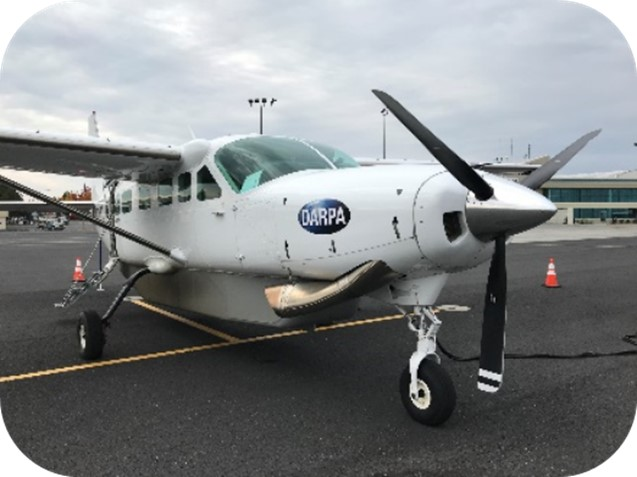
\includegraphics[width=\columnwidth]{figures/caravan.jpg}
	\caption{Boeing Autonomy Testbed Aircraft, Cessna Caravan 208B}
	\label{fig:caravan}
\end{figure}

Detect and avoid (DAA) mission operating and performance standards are defined in RTCA document DO-365 \cite{DO_365}.  The standard provides guidance for interactions of Unmanned Aircraft Systems (UAS) in the National Airspace System, requirements for safe operation of aircraft during encounters including separation distance minimums for remaining well clear of aircraft and avoiding mid-air collisions, and proper aircraft equipage to achieve safe detect and avoid operations.
The assurance challenge posed in our work focuses on the Autonomy Testbed aircraft flying in the vicinity of another ``intruder'' airplane, where the test flight software includes a Boeing-developed LEC to generate an avoidance flight plan for the Testbed to remain well clear of the intruder aircraft as defined in DO-365.  The underlying assurance technology montors the Boeing LEC in order to assess the avoidance trajectory from the LEC and guarantee safety. 

\begin{figure*}
	\centering
	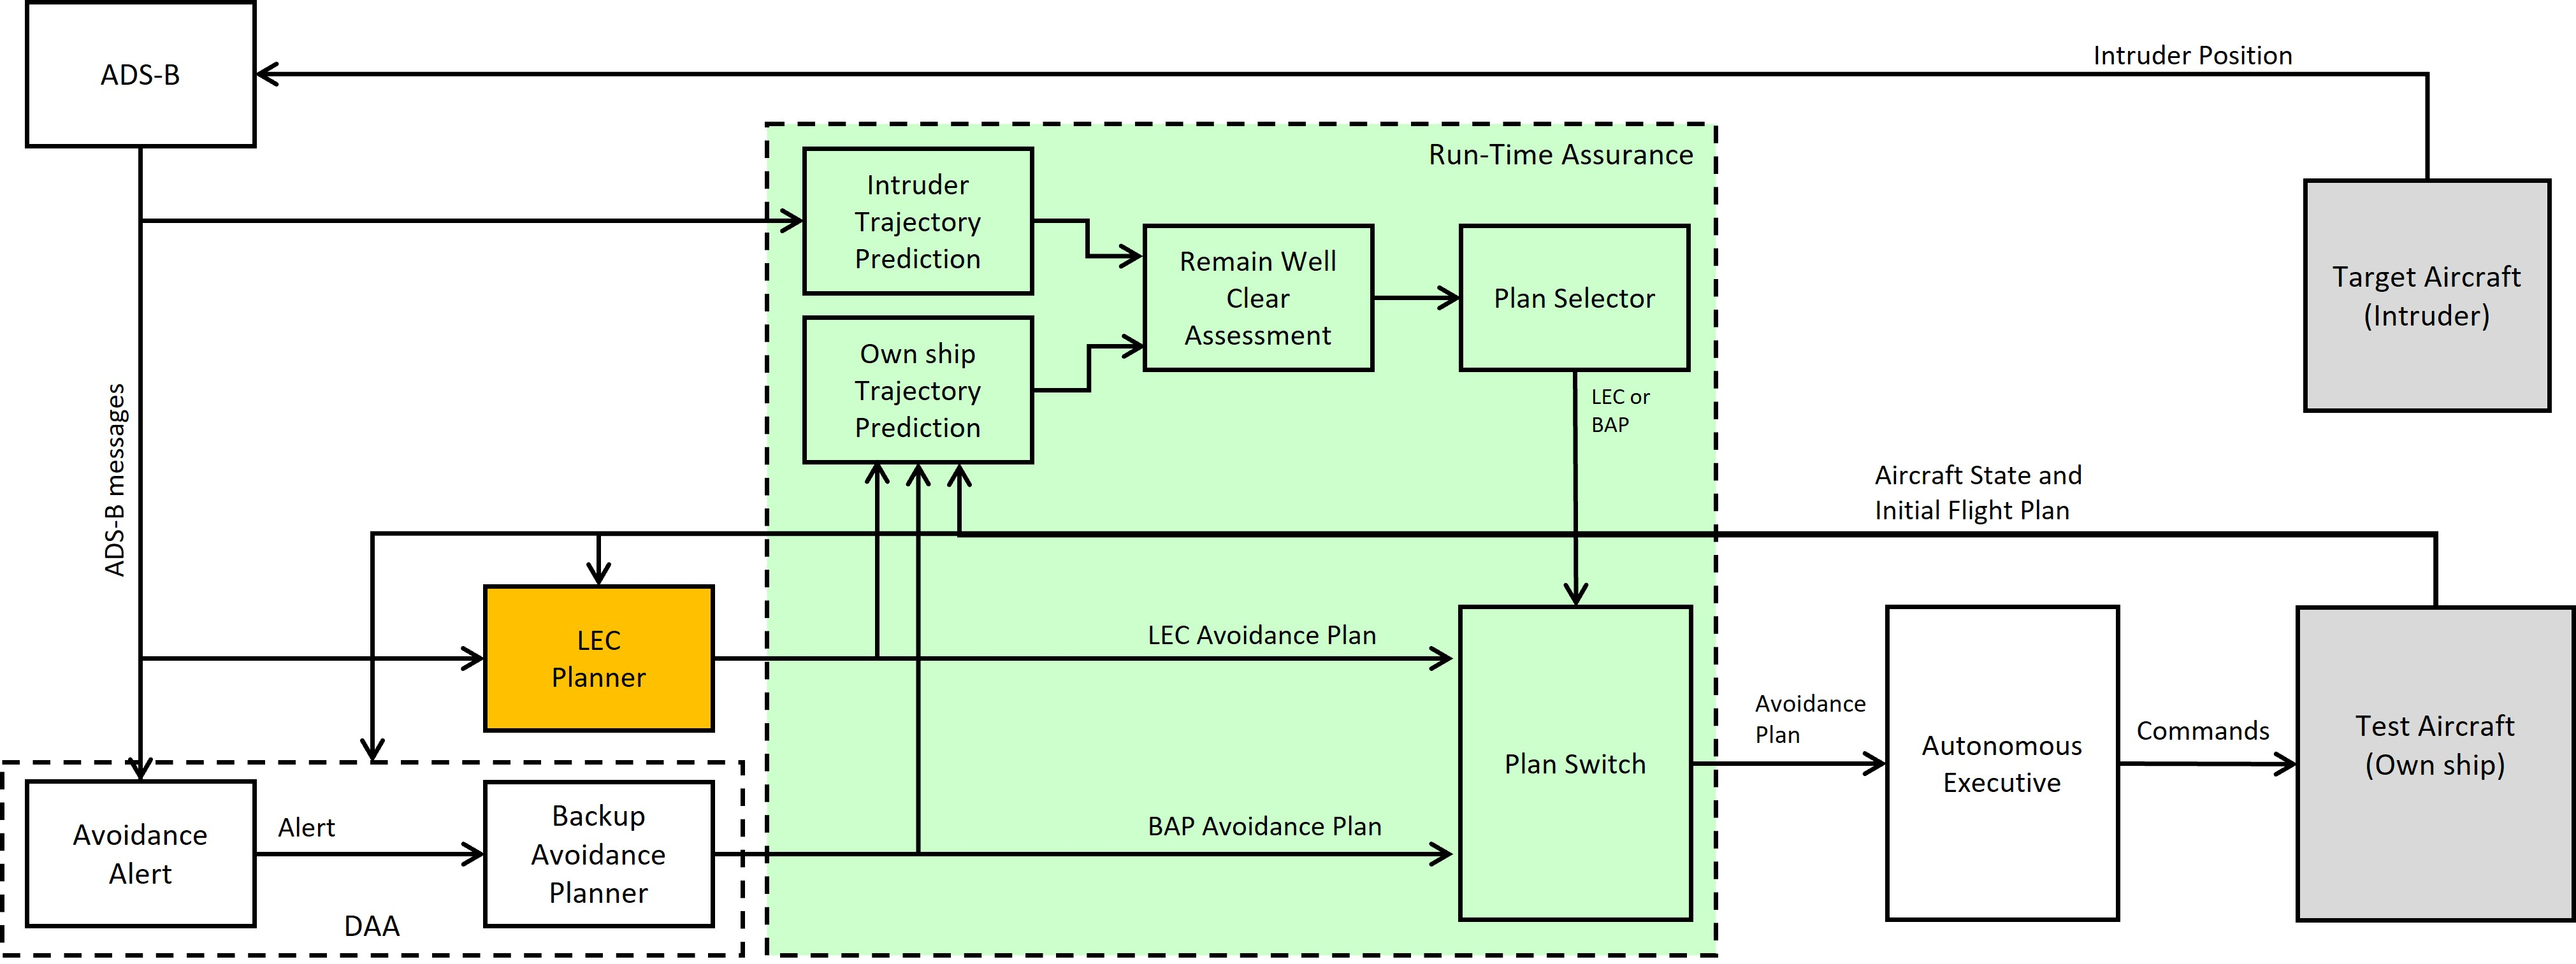
\includegraphics[width=\textwidth]{figures/rta-arch.jpg}
	\caption{Collision avoidance system on the autonomy testbed aircraft with run-time assurance components in green}
	\label{fig:rta-arch}
\end{figure*}

Figure~\ref{fig:rta-arch} shows a block diagram of the autonomy system framework as deployed on the Testbed aircraft.
System elements include: 
\begin{itemize}
\item ADS-B – The primary sensor for perceiving the airspace is the Automated Dependent Surveillance Broadcast (ADS-B) system providing detection information on  nearby aircraft (intruders) to the other system functions.
%\item ADS-B Tracker – Generates intruder track information from received ADS-B messages to the other system functions.
\item Avoidance Alerts – Evaluates potential future traffic conflicts and issues “alerts” to the Avoidance functions.  Assessment definition and requirements are specified in DO-365 MOPS for DAA System.
\item LEC Planner -- Neural network system trained offline through reinforcement learning to generate avoidance flight plans satisfying DAA requirements.  Training and operation is described in the following subsection.  
\item Backup Avoidance Planner – A trusted but less optimal backup planner that provides waypoint navigation paths to avoid airspace incursion.  Avoidance computation method is virtual predictive radar which is designed to provide maximum ``safe passage timed corridors.''  Avoidance path terminates back on the original flight plan.
\item Run-Time Assurance  – Run-time monitoring, predication, and assessment systems that guarantee the selection of a safe flight plan for the aircraft.  Operation and assurance are described in Sections \ref{sec:rta} and \ref{sec:assurance}.
\item Autonomous Executive – Constructs and manages execution of the vehicle flight plan and contains a function to ``splice in'' avoidance guidance waypoint plans into the original flight plan.
%\item Vehicle Manager – Executes flight path provided by AE including guidance and control for the vehicle.  The VM also sends commands and receives feedback from actuation system components.
%\item Actuators / Sensors – Carries out VMS flight control surface commands and provides positional feedback.
%\item Ownship State Estimation – Provides vehicle state information including position, altitude, and speed along with the vehicle inertial reference frame.
%\item Navigation Database – Reference database of aircraft parameters and airspace waypoints, terrain, airports, approaches, etc.  Used for route/avoidance planning purposes.
\end{itemize}

